\documentclass[a4paper,12pt]{article}

\usepackage{preamble}

\title{\vspace{-18mm}\fontsize{18pt}{20pt}\selectfont\textbf{
                    Solução Numérica da Equação de Laplace}} % Título do artigo

\author{
\large
\textsc{Mariana Jó (7241072)}\\
\vspace{-20pt}
}
\date{}

\begin{document}
\maketitle
\thispagestyle{fancy}

\section*{Abstract}

\section{Introdução}

A Equação de Laplace é dada por
\begin{equation}
\nabla^2 \varphi = 0
\label{eq:laplace}
\end{equation}

As soluções para a Equação de Laplace são funções harmônicas. As funções harmônicas
possuem a propriedade do valor médio. Isto é, o valor de $\varphi (x, y, z)$ é a média
do valor ao redor deste ponto. Ou seja, ao desenhar uma bola de raio $R$ entorno do
ponto $(x, y, z)$, a média do valor de $\varphi$ na bola é igual ao valor no centro\cite{grif}:
\begin{equation*}
  \varphi(x, y, z) = \frac{1}{2\pi R}\oint_{\text{esfera}}\varphi \ dS.
\end{equation*}

Esta propriedade das funções harmônicas nos permite resolver a Equação de Laplace
através de métodos de relaxamento. A partir das condições de contorno e "chutes razoáveis" para $\varphi$ nas regiões internas, o valor do potencial para
cada ponto é calculado a partir dos valores de seus vizinhos. Este procedimento é
repetido iterativamente, fazendo com que a solução convirja.

Este trabalho propõe algumas soluções para a Equação de Laplace utilizando métodos de relaxamento.


\section{Problema}


Queremos resolver o potencial dentro de uma caixa em $(x, y, z)$, de lados $(a, b, \infty)$. Ou seja, o problema possui simetria em $z$ e, portanto, basta-nos resolver um problema em duas dimensões, $(x, y)$.

\begin{figure}[H]
\centering
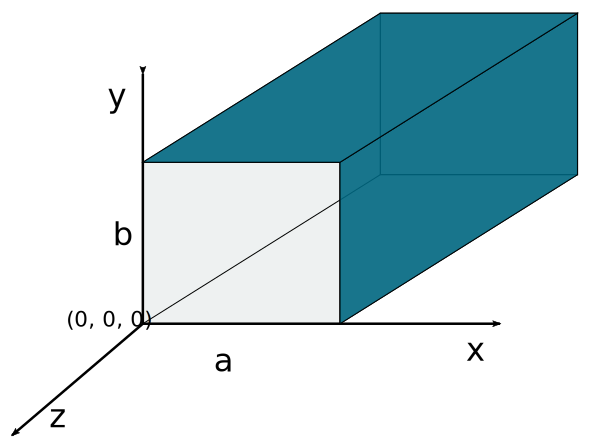
\includegraphics[scale=0.5]{img/box}
  \caption{Geometria do problema.}
\end{figure}

Este problema tem as condições de contorno:
\begin{enumerate}
  \item $\varphi(x,0)=-500V$
  \item $\varphi(x,b)=1000V$
  \item $\varphi(0,y)=0V$
  \item $\varphi(a, y) = 50V$
\end{enumerate}

\section{Discretização e método de relaxamento}

Primeiramente, é necessário discretizar o problema e para isso utilizamos
uma malha\footnote{Traduzido livremente de \textit{mesh grid}.} de pontos que cubra nosso domínio de interesse. Assume-se que
os pontos da malha tenham o mesmo espaçamento $h$ entre si, em todas as
direções.

Cada ponto da malha é descrito pelo par $(i, j)$, assumindo o ponto de
origem $(x, y) = (0, 0)$, onde as coordenadas $(x, y)$ da malha $(i, j)$
são dadas por $x_i=ih$ e $y_j=jh$. Portanto, o objetivo é calcular os valores de $\varphi$ na malha, $\varphi(x_i, y_j) \equiv \varphi_{i, j}$.

O próximo passo é transformar o operador Laplaciano $\nabla^2$ para a versão discreta, ou seja, descrever as derivadas segundas em termos de diferenças finitas.

Consideremos primeiramente apenas a variável $x$:
\begin{equation*}
  \frac{d^2\varphi}{dx^2} = 0
\end{equation*}

Fazendo a expansão de Taylor em $\varphi$ ao redor de $x$ temos:
\begin{equation}
  \varphi(x + h) = \varphi(x)+h\frac{d\varphi}{dx}+\frac{1}{2}h^2\frac{d^2\varphi}{dx^2}+...,
  \label{eq:taylor}
\end{equation}
com todas as derivadas avaliadas no ponto $x$. A (\ref{eq:taylor}) implica
\begin{equation*}
  \varphi(x + h) + \varphi(x - h) = 2\varphi(x)+h^2\frac{d^2\varphi}{dx^2}+\mathcal{O}(h^4).
\end{equation*}

Desconsiderando os termos de maior ordem para um $h$ suficientemente pequeno, podemos reescrever como

\begin{equation}
  \frac{d^2\varphi}{dx^2} \approx \frac{\varphi(x+h)+\varphi(x-h)-2\varphi(x)}{h^2}.
\end{equation}

O desenvolvimento para $y$ é completamente análogo. Assim, combinando as duas soluções, chegamos a uma aproximação para o Laplaciano:
\begin{equation}
  \nabla^2 \varphi = \frac{\varphi(x+h,y)+\varphi(x-h,y)-2\varphi(x,y)}{h^2} +
  \frac{\varphi(x,y+h)\varphi(x,y-h)-2\varphi(x,y)}{h^2}
\end{equation}

Portanto, utilizando a notação sobre a malha, onde $\varphi(x\pm h, y)=\varphi_{i\pm 1,j}$ e $\varphi(x,y\pm h)=\varphi_{i,j\pm 1}$, a Equação de Laplace fica
\begin{equation*}
  \varphi_{i+1, j}+\varphi_{i-1,j}+\varphi_{i,j+1}+\varphi_{i,j-1}-4\varphi_{i,j}=0,
\end{equation*}
podendo ser reescrita como
\begin{equation}
  \varphi_{i,j} = \frac{\varphi_{i+1,j}+\varphi_{i-1,j}+\varphi_{i,j+1}+\varphi_{i,j-1}}{4}.
  \label{eq:num_sol}
\end{equation}

Esta equação é a manifestação da propriedade do valor médio das funções harmônicas. Isto é, o valor em um ponto é a média dos seus valores vizinhos.

De posse desta aproximação, podemos partir de um valor inicial para o potencial, as condições de contorno nas bordas e aplicar (\ref{eq:num_sol}) iterativamente até que se queira, a fim de determinar $\varphi$. Isto é, chagamos assim num método de relaxamento, onde

\begin{equation}
  \varphi_{i,j}^n = \frac{\varphi_{i+1,j}^{n}+\varphi_{i-1,j}^{n}+\varphi_{i,j+1}^{n}+\varphi_{i,j-1}^{n}}{4}.
  \label{eq:num_sol_it}
\end{equation}

Agora, para resolver o problema a partir de (\ref{eq:num_sol_it}) lançaremos mão de dois métodos iterativos: o Método de Jacobi e o Método de Gauss-Seidel.

\subsection*{Método de Jacobi}

DESCRIÇÃO DO MÉTODO

Ao aplicar o este método obtemos a solução

FIGURA DA SOLUÇÃO

O cálculo do erro $\epsilon$ é tal que
\begin{equation}
  \epsilon = \frac{||\mathbf{x}^n-\mathbf{x}^{n-1}||}{||\mathbf{x}^n||} \leq \tau,
  \label{eq:error}
\end{equation}
onde $\tau$ é a tolerância para o erro do método, que é utilizada como critério de parada. O método deve continuar iterando até que a condição em (\ref{eq:error}) seja satisfeita. Para esta solução consideramos $\tau = 10^{-3}$. CITAR REFERENCIA


\subsection*{Método de Gauss-Seidel}

O Método de Gauss-Seidel possui a mesma dinâmica do Método de Jacobi, porém ao invés de utilizar todos os valores da
iteração anterior, os valores disponíveis para $\varphi_{i\pm1, j}$ e $\varphi_{i,j\pm 1}$ são os da própria iteração. Isto torna o processo de relaxamento mais eficiente.

FIGURA DA SOLUÇÃO

Para este método o erro e critério de parada são calculados tal como no Método de Jacobi por (\ref{eq:error}), com a mesma tolerância $\tau$.
\subsection*{Análise de erros}

\section{Solução analítica}

\section{Conclusão}

\begin{thebibliography}{99}

\bibitem[Griffiths, 1999]{grif}
Introduction to electrodynamics, 3rd ed.
\newblock Peason Education.

\end{thebibliography}

\end{document}
